%Template
% !TeX spellcheck = de 
\documentclass[a4paper]{scrartcl}
\usepackage[utf8]{inputenc}
%\usepackage[ngerman]{babel}
\usepackage{geometry,forloop,fancyhdr,fancybox,lastpage}
\usepackage{dsfont}
\usepackage{tikz}
\usepackage[utf8]{inputenc}
%\usepackage[T1]{fontec}
\usepackage{lmodern}
\usepackage{helvet}
\usepackage{geometry}
\usepackage{mathptmx}
\usepackage{amsmath}
\usepackage{amssymb}
\usepackage{graphicx}
\usepackage{tabularx}
\usepackage{ragged2e}
\usepackage{array}
\usepackage[ngerman]{babel}
%\usepackage[table,dvipsnames,svgnames]{xcolor}
\usepackage{lscape}

\usepackage{listings}
\lstset{frame=tb,
	language=Java,
	aboveskip=3mm,
	belowskip=3mm,
	showstringspaces=false,
	columns=flexible,
	basicstyle={\small\ttfamily},
	numbers=left,
	numberstyle=\tiny\color{gray},
	keywordstyle=\color{blue},
	commentstyle=\color{dkgreen},
	stringstyle=\color{mauve},
	breaklines=true,
	breakatwhitespace=true,
	tabsize=3
}
\geometry{a4paper,left=3cm, right=3cm, top=3cm, bottom=3cm}
% Diese Daten müssen pro Blatt angepasst werden:
\newcommand{\NUMBER}{6}
\newcommand{\EXERCISES}{3}
% Diese Daten müssen einmalig pro Vorlesung angepasst werden:
\newcommand{\COURSE}{Stochastik}
\newcommand{\TUTOR}{TBD}
\newcommand{\STUDENTA}{Stefan Wezel}
\newcommand{\STUDENTB}{Stefan Wezel}
\newcommand{\STUDENTC}{}
\newcommand{\DEADLINE}{07.06.2018}




%Math
\usepackage{amsmath,amssymb,tabularx}

%Figures
\usepackage{graphicx,tikz,color,float}
\graphicspath{ {home/stefan/picures/} }
\usetikzlibrary{shapes,trees}

%Algorithms
\usepackage[ruled,linesnumbered]{algorithm2e}

%Kopf- und Fußzeile
\pagestyle {fancy}
\fancyhead[L]{\STUDENTA}
\fancyhead[C]{\COURSE}
\fancyhead[R]{\today}

\fancyfoot[L]{}
\fancyfoot[C]{}
\fancyfoot[R]{Seite \thepage}

%Formatierung der Überschrift, hier nichts ändern
\def\header#1#2{
	\begin{center}
		{\Large\bf Übungsblatt #1}\\
		{(Abgabetermin #2)}
	\end{center}
}

%Definition der Punktetabelle, hier nichts ändern
\newcounter{punktelistectr}
\newcounter{punkte}
\newcommand{\punkteliste}[2]{%
	\setcounter{punkte}{#2}%
	\addtocounter{punkte}{-#1}%
	\stepcounter{punkte}%<-- also punkte = m-n+1 = Anzahl Spalten[1]
	\begin{center}%
		\begin{tabularx}{\linewidth}[]{@{}*{\thepunkte}{>{\centering\arraybackslash} X|}@{}>{\centering\arraybackslash}X}
			\forloop{punktelistectr}{#1}{\value{punktelistectr} < #2 } %
			{%
				\thepunktelistectr &
			}
			#2 &  $\Sigma$ \\
			\hline
			\forloop{punktelistectr}{#1}{\value{punktelistectr} < #2 } %
			{%
				&	
			} &\\
			\forloop{punktelistectr}{#1}{\value{punktelistectr} < #2 } %
			{%
				&
			} &\\
		\end{tabularx}
	\end{center}
}

\begin{document}

\section*{Aufgabe 9}
Wir können folgenden Wahrscheinlichkeitsraum benutzen:\\\\
$
\Omega = \lbrace 
	\text{rot ohne Aufdruck}, 
	\text{rot mit Aufdruck},\\
	\text{grün ohne Aufdruck},
	\text{grün mit Aufdruck},\\
	\text{blau ohne Aufdruck},
	\text{blau mit Aufdruck}
	\rbrace
\\\\ %TODO doesn't sum up to 1
\mathcal{F} = \mathcal{P}(\Omega)\\\\
P = \lbrace
	P(\emptyset) = 0,\\
	P(\text{rot ohne Aufdruck}) = \frac{3}{10} \cdot \frac{9}{10} = \frac{27}{100},\\
	P(\text{rot mit Aufdruck}) = \frac{3}{10} \cdot \frac{1}{10}  = \frac{3}{100},\\
	P(\text{blau ohne Aufdruck}) = \frac{3}{10} \cdot \frac{9}{10}  = \frac{27}{50},\\
	P(\text{blau mit Aufdruck}) = \frac{3}{10} \cdot \frac{1}{10}  = \frac{3}{50},\\
	P(\text{grün ohne Aufdruck}) = \frac{4}{10} \cdot \frac{8}{10}  = \frac{32}{100},\\
	P(\text{grün mit Aufdruck}) = \frac{4}{10} \cdot \frac{2}{10}  = \frac{8}{100},\\
	P(\Omega) = 1
	\rbrace
\\\\
... = (\Omega, \mathcal{F}, P)
$
\\\\
Nach dem Theorem von Bayes können wir für die Wahrscheinlichkeit, dass eine gezogene Kugel rot ist, unter Annahme des Priors, dass sie ein Aufdruck besitzt folgende Gleichung aufstellen:\\\\
$
P(Rot|Aufdruck) \Leftrightarrow \frac{P(Aufdruck|Rot) \cdot P(Rot)}{P(Aufdruck)}\\\\
\Leftrightarrow \frac{P(Aufdruck|Rot) \cdot P(Rot)}{P(Aufdruck|Rot) \cdot P(Rot) + P(Aufdruck|Blau) \cdot P(Blau) + P(Aufdruck|Gruen) \cdot P(Gruen)}\\\\
\Leftrightarrow \frac{\frac{1}{10} \cdot \frac{3}{10}}{\frac{1}{10} \cdot \frac{3}{10} + \frac{1}{10} \cdot \frac{3}{10} + \frac{2}{10} \cdot \frac{4}{10}}\\\\
\Leftrightarrow \frac{\frac{3}{100}}{\frac{3}{100} + \frac{3}{100} + \frac{8}{100}}\\\\
\Leftrightarrow \frac{\frac{3}{100}}{\frac{14}{100}}\\\\
\Leftrightarrow \frac{300}{1400}\\\\
\Leftrightarrow \frac{3}{14}
$


\section*{Aufgabe 10}
\subsection*{(a)}
Die Zahlen stehen jeweils für die Anzahl der gewürfelten Augen. Die Wahrscheinlichkeit einer Summe ergibt sich aus den aufsummierten Wahrscheinlichkeiten der möglichen Kombinationen.
\newpage$
P(2) = P(1) \cdot P(1) = \frac{1}{6} \cdot \frac{1}{6} = \frac{1}{36}\\\\
P(3) = 2 \cdot P(2) \cdot P(1) =2 \cdot\frac{1}{6} \cdot \frac{1}{6} =\frac{2}{36}= \frac{1}{18}\\\\
P(4) = P(2) \cdot + P(2) + P(3) \cdot P(1) \cdot 2 = \frac{1}{6} \cdot \frac{1}{6} + \frac{1}{6} \cdot \frac{1}{6} \cdot 2 = \frac{1}{36} + \frac{2}{36} = \frac{3}{36} = \frac{1}{12}\\\\
P(5) = 2 \cdot P(1) \cdot P(1) + 2 \cdot P(3)\cdot P(2) = 2 \cdot \frac{1}{36} +2 \cdot \frac{1}{36} = \frac{4}{36} = \frac{1}{9}\\\\
P(6) = 2 \cdot P(5) \cdot P(1) + 2 \cdot P(4) \cdot P(2) + P(3) \cdot P(3) = \frac{2}{36} + \frac{2}{36} + \frac{1}{36} = \frac{5}{36}\\\\
P(7) = 2 \cdot P(6) \cdot P(1) + 2 \cdot P(5) \cdot P(2) +2 \cdot P(4) \cdot P(3) = 2 \cdot \frac{1}{36} + 2 \cdot \frac{1}{36} + 2 \cdot \frac{1}{36} = \frac{6}{36} = \frac{1}{6}\\\\
P(8) = 2 \cdot P(6) \cdot P(2) + 2 \cdot P(5) \cdot P(3) + P(4) \cdot P(4) = \frac{2}{36} + \frac{2}{36} + \frac{1}{36} = \frac{5}{36}\\\\
P(9) = 2 \cdot P(5) \cdot P(4) + 2 \cdot P(6)\cdot P(3) = 2 \cdot \frac{1}{36} +2 \cdot \frac{1}{36} = \frac{4}{36} = \frac{1}{9}\\\\
P(10) = 2 \cdot P(6) \cdot P(4) + P(5) \cdot P(5) = \frac{2}{36} +  \frac{1}{36} = \frac{3}{36} = \frac{1}{12}\\\\
P(11) = 2 \cdot P(5) \cdot P(6) = 2 \cdot \frac{1}{6} \cdot \frac{1}{6} = \frac{2}{36} = \frac{1}{18}\\\\
P(12) = P(6) \cdot P(6) = \frac{1}{6} \cdot \frac{1}{6} = \frac{1}{36}
$

\subsection*{(b)}
Wir mit einem Würfel an und fügen dann falls benötigt neue Augenzahlen hinzu um die drei freien Flächen zu füllen.\\
Stimmen die Wahrscheinlichkeiten mit der, der vorherigen Teilaufgabe überein (also wenn $p_k = q_k$), sind sie mit einem $\checkmark$ markiert.
\\
\\
$
P(2) = P(1) \cdot P(1) = \frac{1}{3} \cdot \frac{1}{12} = \frac{1}{36} \checkmark\\\\
P(3) = P(1) \cdot P(2) \cdot 2= \frac{1}{3} \cdot \frac{1}{12} \cdot 2 = \frac{2}{36} = \frac{1}{18} \checkmark\\\\
P(4) = P(1) \cdot P(3) \cdot 2 + P(2) \cdot P(2) = \frac{1}{3} \cdot \frac{1}{12} \cdot 2 + \frac{1}{3} \cdot \frac{1}{12}=\frac{2}{36} \frac{1}{36} = \frac{3}{36} = \frac{1}{12} \checkmark\\\\
P(5) = P(1) \cdot P(4) + P(2) \cdot P(3) \cdot 2 = \frac{1}{36} + \frac{2}{36} = \frac{3}{36} \\
\Rightarrow \text{Eine weitere 4 wird benoetigt. Dann: } \frac{1}{3} \cdot \frac{2}{12} + \frac{2}{36} = \frac{4}{36} =\frac{1}{9}\checkmark\\\\
P(6) = P(1) \cdot P(5) + P(2) \cdot P(4) + P(3) \cdot P(3) = \frac{1}{36} \cdot \frac{2}{36} \cdot \frac{1}{36} = \frac{4}{36}\\
\Rightarrow \text{Eine weitere 5 wird benoetigt. Dann: } \frac{2}{36} + \frac{2}{36} + \frac{1}{36} = \frac{5}{36}\checkmark\\\\
P(7) = P(1) \cdot P(6) + P(2) \cdot P(5) + P(3) \cdot P(4) = \frac{1}{36} + \frac{2}{26} + \frac{2}{36} = \frac{5}{36}\\
\Rightarrow \text{Eine weitere 6 wird benoetigt. Dann: } \frac{2}{36} + \frac{2}{36} + \frac{2}{36} = \frac{6}{36} = \frac{1}{6}\checkmark\\\\
\text{Jetzt sind nur noch 3 Felder übrig... hoffen wir also, dass es reicht...}\\
\\
P(8) = P(1) \cdot P(7) + P(2) \cdot P(6) + P(3)\cdot P(5) = \frac{1}{36} + \frac{2}{36} + \frac{2}{36} = \frac{5}{36} \text{Juhu!} \checkmark\\\\
P(9) = P(1) \cdot P(8) + P(2) \cdot P(7) + P(3) \cdot P(6) = \frac{1}{36} + \frac{1}{36} + \frac{1}{36} + \frac{2}{36} = \frac{4}{36} = \frac{1}{9}\checkmark\\\\
P(10) = P(1) \cdot P(9) + P(2) \cdot P(8) + P(3) \cdot P(7) = \frac{1}{36} + \frac{1}{36}+\frac{1}{36} = \frac{3}{36} = \frac{1}{12} \checkmark\\\\
P(11) = P(2) \cdot P(9) + P(2) \cdot P(9) = \frac{1}{36} + \frac{1}{36} = \frac{2}{36} = \frac{1}{18} \checkmark\\\\
P(12) = P(3) \cdot P(9) = \frac{1}{3} \cdot \frac{1}{12} = \frac{1}{36} \checkmark
$
\\
\\
Daraus resultiert ein Dodekaeder mit folgenden Augenzahlen:\\\\
\begin{tabular}{|c|c|c|c|}
	\hline 
	1 & 2 & 3 & 4 \\ 
	\hline 
	4 & 5 & 5 & 6 \\ 
	\hline 
	6 & 7 & 8 & 9 \\ 
	\hline 
\end{tabular} 
\\
\\
\section*{Aufgabe 11}
\subsection*{(a)}
Siehe letzte Seite



\subsection*{(b)}
Um die Wahrscheinlichkeiten für die einzelnen Allelkombinationen zu bekommen summieren wir die Wahrscheinlichkeiten der jeweiligen Blätter des Baumes auf.\\\\
\begin{align*}
	P(AA) &= p^2 + \frac{1}{2} \cdot p \cdot q + \frac{1}{2} \cdot p \cdot q + \frac{1}{4} \cdot q^2\\
	&=p^2 + pq + \frac{1}{4} q^2\\
	\\
	P(Aa) &= \frac{1}{2} \cdot p \cdot q + \frac{1}{2} \cdot q \cdot q + \frac{1}{4} \cdot q^2 + \frac{1}{4} \cdot q^2 + \frac{1}{2} \cdot q \cdot r + r \cdot p + \frac{1}{2} \cdot q \cdot r\\
	&= 2 \cdot p \cdot r  +p \cdot q + \frac{1}{2} \cdot q^2 + q \cdot r\\
	\\
	P(aa) &= \frac{1}{4}\cdot q^2 +\frac{1}{2} \cdot q \cdot r + \frac{1}{2} \cdot q \cdot r + r^2\\
	&= \frac{1}{4}\cdot q^2 +  q \cdot r + r^2
\end{align*}
\newpage

\subsection*{(c)}
Hierzu setzen wir die Wahrscheinlichkeiten in die Gleichungen für die jeweiligen Genotypen des Kindes ein und schauen, ob sie denen der Eltern entsprechen...\\
\\
\begin{align*}
P(AA) &= x^4 + x^2 \cdot 2x(1-x) + \frac{1}{4} \cdot (2x \cdot(1-x)^2)^2\\
&= x^4 + x^2(2x-2x^2) + \frac{1}{4} \cdot (4x^2 - 2 \cdot 2x \cdot 2x^2 + 4x^4)\\
&=x^4 + 2x^3 - 2x^4 + \frac{1}{4} \cdot (4x^2 - 8x^3 + 4x^4)\\
&=x^4 + 2x^3 - 3x^4 + x^2 - 2x^3 + x^4\\
&=x^2 \text{ ..stimmt überein   }\checkmark 
\end{align*}

\begin{align*}
P(Aa) &= 2x^2 \cdot (1-x)^2 + x^2(2x(1-x)) + \frac{1}{2}(2x(1-x))^2 + 2x(1-x) \cdot (1-x)\\
&= 2x^2(1-2x+x^2) + x^2(2x-2x^2) + \frac{1}{2}(2x-2x^2)^2 + (2x-2x^2)\cdot(1-2x+x^2)\\
&= 2x^2 - 4x^3 + 2x^4 + 2x^3 -2x^4 + \frac{1}{2} (4x^2 -8x^3 + 4x^4) + (2x-2x^2) \cdot (1-2x + x^2)\\
&= 2x^2 -2x^3 + 2x^2 - 4x^3 + 2x^4 + 2x - 4x^2 + 2x^3 - 2x^2 + 4x^3 -2x^4\\
&=-2x^2 + 2x\\
&=2x\cdot(1-x) \checkmark
\end{align*}


\begin{align*}
P(Aa) &= \frac{1}{4} \cdot (2x - 2x^2)^2 + (2x-2x^2) (1-x)^2 + (1-x)^4\\
&=\frac{1}{4} (4x^2 - 8x^3 + 4x^4) + (2x-2x^2)(1-2x + x^2) + ((1-x)^2)^2\\
&=x^2 - 2x^3 + x^4 + 2x - 4x^2 + 2x^3 - 2x^2 + 4x^3 -2x^4 + (1-2x+x^2)(1-2x+x^2)\\
&=-5x^2 + 4x^3 -x^4 + 2x +1-2x + x^2 -2x + 4x^2 -2x^3 + x^2 -2x^3 + x^4\\
&=1-2x + x^2\\
&=(1-x)^2 \checkmark
\end{align*}






\newpage
\begin{landscape}
	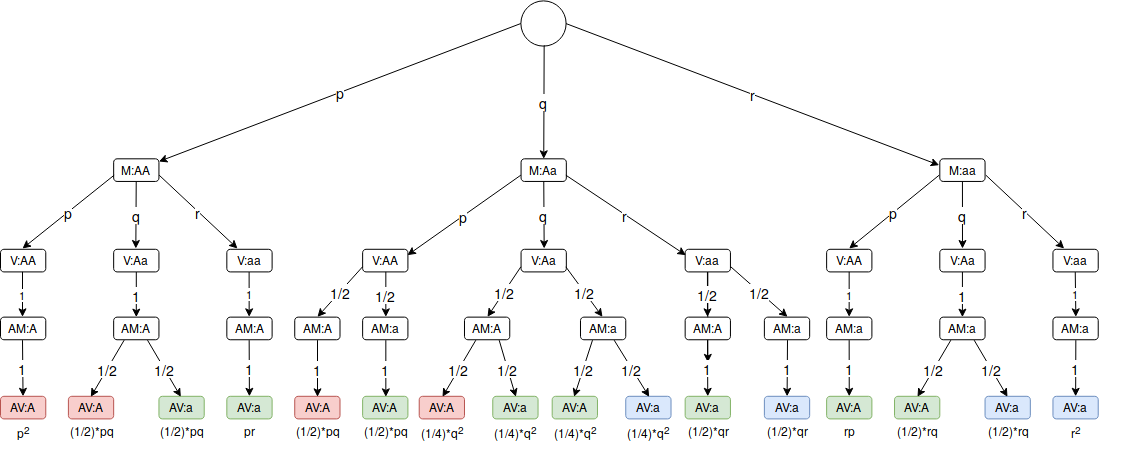
\includegraphics[height=9cm,width=22cm]{stocha_blatt3_3a.png}
	%\caption{Aufgabe 3 (a)}
\end{landscape}
















\end{document}
